% Drawing 148/04-2 -- folder 148, batch 04, archive page 71 (PDF page 72).
% Transcription: page de dessin, qui revient au découpage en pantalons des pages 66-69
% Kind: triangulated map with nested pants curves; weighted trivalent graph. Method 2 (schematic redraw from the facsimile). Status: partial.
% Notes: Whole half-page. Left: a triangulation with eleven ringed vertices and half-lines going off, surrounded by about ten nested closed curves (the pants decomposition curves, schematised as concentric rings, and only seven drawn); the edges are read approximately. Right: a trivalent graph with weights (1 9, 7, 1, 25, 17 in ink; small figures 2, 3, 4, 5, 6 and ringed 1, 2, 3 in pencil), a loop at 17 and free edges, one with an arrow. Caption: "decoupages pantalonesques d'une carte (triangulee)". The small weights are tiny and placed approximately.
% Coordinates: 1 unit = 1 mm = 1/100 of the crop width (bbox in page fractions: [0.03, 0.04, 0.97, 0.53]).
% Redrawn by Claude (claude-opus-5-5), issue #73, 2026-11-07; not checked by a human; not compiled (no TeX in the session).
% Rights: reproduces part of the work -- behind RENDER_TRANSCRIPTS, never published by itself.
\documentclass[tikz,border=3pt]{standalone}
\usepackage{amsmath,amssymb}
\usetikzlibrary{patterns,arrows.meta}
\tikzset{pencil/.style={black!45}, struck/.style={black!35}, mark/.style={circle,draw,inner sep=1.3pt}, pt/.style={circle,fill,inner sep=0.9pt}, opt/.style={circle,draw,fill=white,inner sep=1.1pt}}
\begin{document}
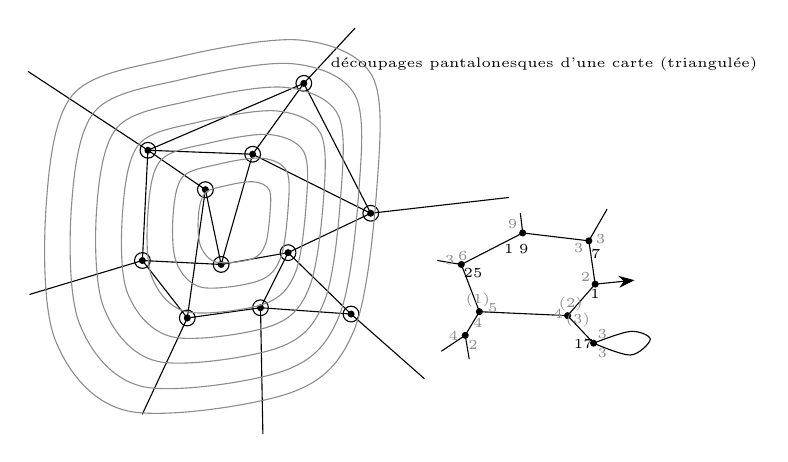
\begin{tikzpicture}[x=1mm,y=1mm,line cap=round,line join=round,font=\scriptsize]
\draw (30.7,-23) -- (44,-23.5);
\draw (30.7,-23) -- (38,-28);
\draw (38,-28) -- (40,-37.5);
\draw (44,-23.5) -- (40,-37.5);
\draw (44,-23.5) -- (50.5,-14.5);
\draw (50.5,-14.5) -- (59,-31);
\draw (44,-23.5) -- (59,-31);
\draw (30,-37) -- (40,-37.5);
\draw (40,-37.5) -- (48.5,-36);
\draw (48.5,-36) -- (59,-31);
\draw (30.7,-23) -- (30,-37);
\draw (30,-37) -- (35.7,-44.3);
\draw (35.7,-44.3) -- (45,-43);
\draw (45,-43) -- (56.5,-43.8);
\draw (45,-43) -- (48.5,-36);
\draw (56.5,-43.8) -- (48.5,-36);
\draw (38,-28) -- (35.7,-44.3);
\draw (30.7,-23) -- (50.5,-14.5);
\draw (30.7,-23) circle[radius=1];
\draw (44,-23.5) circle[radius=1];
\draw (50.5,-14.5) circle[radius=1];
\draw (38,-28) circle[radius=1];
\draw (59,-31) circle[radius=1];
\draw (30,-37) circle[radius=1];
\draw (40,-37.5) circle[radius=1];
\draw (48.5,-36) circle[radius=1];
\draw (35.7,-44.3) circle[radius=1];
\draw (45,-43) circle[radius=1];
\draw (56.5,-43.8) circle[radius=1];
\node[pt] at (30.7,-23) {};
\node[pt] at (44,-23.5) {};
\node[pt] at (50.5,-14.5) {};
\node[pt] at (38,-28) {};
\node[pt] at (59,-31) {};
\node[pt] at (30,-37) {};
\node[pt] at (40,-37.5) {};
\node[pt] at (48.5,-36) {};
\node[pt] at (35.7,-44.3) {};
\node[pt] at (45,-43) {};
\node[pt] at (56.5,-43.8) {};
\draw (15.5,-13) -- (30.7,-23);
\draw (15.7,-41.3) -- (30,-37);
\draw (59,-31) -- (76.5,-29);
\draw (30,-56.5) -- (35.7,-44.3);
\draw (50.5,-14.5) -- (57,-7.5);
\draw (45.3,-59) -- (45,-43);
\draw (65.8,-52) -- (56.5,-43.8);
\draw[pencil] plot[smooth cycle, tension=0.55] coordinates {(37.1,-31.5) (37.9,-28.5) (40.6,-27.5) (44.1,-27) (46.1,-28) (46.2,-31) (45.6,-35) (43.9,-36.8) (39.4,-37.2) (37.4,-35.2)};
\draw[pencil] plot[smooth cycle, tension=0.55] coordinates {(33.9,-31.2) (35.1,-26.4) (39.5,-24.8) (45.1,-24) (48.3,-25.6) (48.5,-30.4) (47.5,-36.8) (44.7,-39.6) (37.5,-40.4) (34.3,-37.2)};
\draw[pencil] plot[smooth cycle, tension=0.55] coordinates {(30.7,-30.9) (32.3,-24.3) (38.4,-22.1) (46.1,-21) (50.5,-23.2) (50.8,-29.8) (49.4,-38.6) (45.5,-42.5) (35.6,-43.5) (31.2,-39.1)};
\draw[pencil] plot[smooth cycle, tension=0.55] coordinates {(27.5,-30.6) (29.6,-22.2) (37.2,-19.4) (47,-18) (52.6,-20.8) (53,-29.2) (51.2,-40.4) (46.4,-45.3) (33.8,-46.7) (28.1,-41.1)};
\draw[pencil] plot[smooth cycle, tension=0.55] coordinates {(24.2,-30.3) (26.8,-20.1) (36.1,-16.7) (48,-15) (54.8,-18.4) (55.2,-28.6) (53.1,-42.2) (47.2,-48.1) (31.9,-49.8) (25.1,-43)};
\draw[pencil] plot[smooth cycle, tension=0.55] coordinates {(21,-30) (24,-18) (35,-14) (49,-12) (57,-16) (57.5,-28) (55,-44) (48,-51) (30,-53) (22,-45)};
\draw[pencil] plot[smooth cycle, tension=0.55] coordinates {(17.8,-29.7) (21.2,-15.9) (33.9,-11.3) (50,-9) (59.2,-13.6) (59.8,-27.4) (56.9,-45.8) (48.8,-53.8) (28.1,-56.1) (18.9,-47)};
\draw (78.3,-33.5) -- (70.5,-37.5);
\draw (78.3,-33.5) -- (86.7,-34.5);
\draw (86.7,-34.5) -- (87.5,-40);
\draw (87.5,-40) -- (84,-44);
\draw (84,-44) -- (72.8,-43.5);
\draw (72.8,-43.5) -- (70.5,-37.5);
\draw (72.8,-43.5) -- (71,-46.5);
\draw (84,-44) -- (87.3,-47.5);
\draw plot[smooth, tension=0.55] coordinates {(87.3,-47.5) (92,-46) (94.5,-47) (92,-49) (87.3,-47.5)};
\draw (78.3,-33.5) -- (78,-31);
\draw (86.7,-34.5) -- (89,-30.5);
\draw[-{Stealth[length=2mm]}] (87.5,-40) -- (92.5,-39.5);
\draw (70.5,-37.5) -- (67.5,-37);
\draw (71,-46.5) -- (68,-48.5);
\draw (71,-46.5) -- (71.5,-49.5);
\node[pt] at (78.3,-33.5) {};
\node[pt] at (86.7,-34.5) {};
\node[pt] at (87.5,-40) {};
\node[pt] at (84,-44) {};
\node[pt] at (72.8,-43.5) {};
\node[pt] at (70.5,-37.5) {};
\node[pt] at (71,-46.5) {};
\node[pt] at (87.3,-47.5) {};
\node[inner sep=1pt] at (77.5,-35.5) {\tiny $1\;9$};
\node[inner sep=1pt] at (87.6,-36.2) {\tiny $7$};
\node[inner sep=1pt] at (87.5,-41.2) {\tiny $1$};
\node[inner sep=1pt] at (72,-38.6) {\tiny $25$};
\node[inner sep=1pt] at (86,-47.6) {\tiny $17$};
\node[inner sep=1pt,pencil] at (77,-32.4) {\tiny $9$};
\node[inner sep=1pt,pencil] at (85.4,-35.4) {\tiny $3$};
\node[inner sep=1pt,pencil] at (88.2,-34.3) {\tiny $3$};
\node[inner sep=1pt,pencil] at (86.3,-39.1) {\tiny $2$};
\node[inner sep=1pt,pencil] at (70.7,-36.4) {\tiny $6$};
\node[inner sep=1pt,pencil] at (69,-37) {\tiny $3$};
\node[inner sep=1pt,pencil] at (72.6,-42) {\tiny $(1)$};
\node[inner sep=1pt,pencil] at (74.5,-43) {\tiny $5$};
\node[inner sep=1pt,pencil] at (72.6,-45) {\tiny $4$};
\node[inner sep=1pt,pencil] at (69.5,-46.6) {\tiny $4$};
\node[inner sep=1pt,pencil] at (72,-47.7) {\tiny $2$};
\node[inner sep=1pt,pencil] at (82.8,-43.8) {\tiny $4$};
\node[inner sep=1pt,pencil] at (84.4,-42.5) {\tiny $(2)$};
\node[inner sep=1pt,pencil] at (85.3,-44.6) {\tiny $(3)$};
\node[inner sep=1pt,pencil] at (88.4,-46.4) {\tiny $3$};
\node[inner sep=1pt,pencil] at (88.4,-48.7) {\tiny $3$};
\node[inner sep=1pt] at (81,-12) {\tiny découpages pantalonesques d'une carte (triangulée)};
\end{tikzpicture}
\end{document}
